\section{HARDWARE DESIGN}
For this section and phase of the project, the next steps were done:
\begin{itemize}
    \item Analyzing the hardware elements.
    \item Analyze the connections needed.
    \item Select the pin connections for every element.
    \item Mount the system.
\end{itemize}
This approach led to a faster design of the solution.
\subsection{Hardware elements}
For the development of the project, all the hardware elements were identified and studied to obtain information of all the possible utilities that the system could use.
\begin{itemize}
    \item \textbf{DISCO-L072CZ-LRWAN1}\cite{DISCOL072CZLRWAN1Mbeda}: This embedded platform integrates the \texttt{STM32L072CZ}\cite{STM32L072CZUltralowpowerArm} cortex M0+ chip. This platform 
    focuses on the connectivity of the system. It provides:
    \begin{itemize}
        \item 192KB of flash memory.
        \item 20KB of RAM.
        \item USER and RESET button.
        \item \acrshort{i2c} and \acrshort{uart} connections.
        \item 16 bit timers along with LowPower timers.
        \item Low Power modes.
        \item A SX1276 transceiver that will be used to implement LoraWan communications on the next subject.
    \end{itemize}
    \item \textbf{I2C Accelerometer}\cite{MMA8451Q1a}: This sensor by Freescale, integrated by Adafruit\cite{DownloadsAdafruitMMA8451} offers 
    a 14 bit triple-axis accelerometer, as well as a  interruptions for events such as freefall and motion detection, transient detection, orientation changes and tap detections.\newline
    It also provides low power modes and deep configuration for sensibility.
    \item \textbf{I2C Color Sensor}\cite{TCS34725}: This chip by \acrfullr{taos} is integrated in a breakout board by Adafruit\cite{RGBColorSensor}. It consist on a 3 by 4 photodiode array with configurable integrators. 
    \newline It provides readings for clear, red, green and blue values in a 16 bit format. It also provides configuration for integration time, automatic readings and configurable interruptions for limits on the clear value.
    \item \textbf{I2C Temperature and Humidity Sensor}\cite{Support_Documents_TechnicalDocs_Si7021A20}: This chip by Silicon Labs is integrated in a breakout board by Adafruit. It allows readings of relative humidity and temperature of the air.
    \item \textbf{UART GPS}\cite{GlobalTopFGPMMOPA6HDatasheetV0A}: This GPS sensor with the integration from Adafruit\cite{gpsDownloadsAda} provides real time information about location following the \acrfullr{nmea} data standard.
    \item \textbf{SEN-13322 Analog Soil Moisture Sensor}\cite{SparkFunSoilMoisture}: This sensor by SparkFun allows to read the moisture level between the two pads.
    \item \textbf{RGB Led}: A common anode RGB led.
    \item \textbf{Phototransistor}\cite{HW5P1_2015__1_}: This element allows for the reading of the brightness in the environment.
\end{itemize}
\clearpage
\subsection{Block Diagram}
To design the solution, the diagram in \autoref{fig:proposedBlock} identifies the main blocks and hardware interfaces needed. The left side and the GPS include 5V powered elements, and the right side contains 3.3V elements.
\begin{figure}[H]
    \centering
    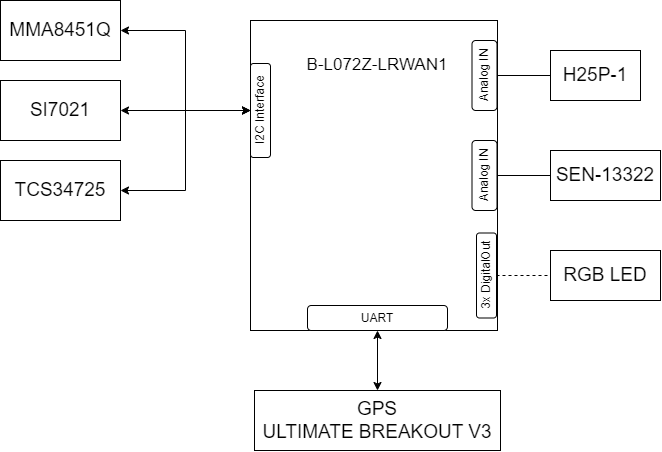
\includegraphics[width=0.6\textwidth]{images/3/General.drawio.png}
    \caption{Block identification for the hardware connections}
    \label{fig:proposedBlock}
\end{figure}

Next, the selection of the connections to the L072CZ were done in the next order: \acrshort{i2c}, \acrshort{uart}, analog connections and finally DigitalOut connections. It is important to note that, as we needed to indicate the working mode with the board leds, we can't 
use the pins connected directly to those elements.
\begin{itemize}
    \item For the I2C, the \acrfullr{mcu} offers 3 options, I2C1,I2C2 and I2C3, being the second one the worst in terms of capabilities.For this system and this use case, I2C1 was selected because, as seen in \autoref{fig:communications}, its the interface with less conflicts.
    \item For the Serial interface to communicate with the GPS, the options are \texttt{USART1}, \texttt{USART2}, \texttt{USART4} and \texttt{USART5}, with the last two having less capabilities. In this case, the L072CZ really only offers the first two, but the \texttt{USART2} 
    is used as a virtual COM port with the ST-Link. The selection was the \texttt{USART1}, also, as can be seen in \autoref{fig:communications}, it has the least conflicts of all.
    \item For the analog sensors, the \texttt{PA\_0} and \texttt{PA\_4} pins were selected, as we only need two Analog IN connections.
\end{itemize}

\begin{figure}[H]
    \centering
    \begin{subfigure}[t]{0.45\textwidth}
        \centering
        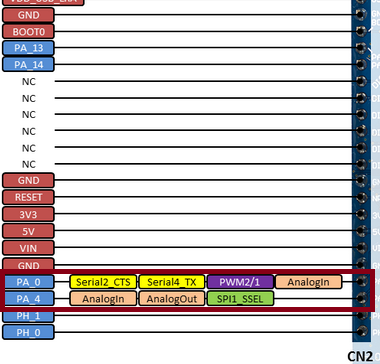
\includegraphics[width=0.66\textwidth]{images/3/Analog.png}
        \caption{Analog selection}
    \end{subfigure}
    \begin{subfigure}[t]{0.45\textwidth}
        \centering
        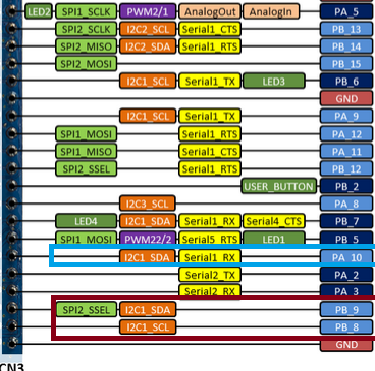
\includegraphics[width=0.66\textwidth]{images/3/I2CSerial.png}
        \caption{I2C and UART selection}
    \end{subfigure}
    \caption{Communication interfaces selection}
    \label{fig:communications}
\end{figure}
\clearpage
At last, the final DigitalOut connections were defined. The final connections for every element are defined in the next tables.
\begin{table}[H]
    \begin{center}
        \begin{tabular}{|p{0.20\textwidth} | p{0.20\textwidth} | p{0.20\textwidth}| p{0.20\textwidth}|}
            \hline
            \textbf{Sensor} & \textbf{Sensor Pin} & \textbf{L072CZ connector} & \textbf{L072CZ Pin name}\\
            \hline
            H25P-1 & SIG & CN2\_24 & PA\_4 \\
            \hline
            SEN-13322 & SIG & CN2\_23 & PA\_0 \\
            \hline
            RGB Led & RED & CN2\_23 & PA\_0 \\%TODO
            \hline
            RGB Led & GREEN & CN2\_23 & PA\_0 \\
            \hline
            RGB Led & BLUE & CN2\_23 & PA\_0 \\
            \hline
             & GND & CN2\_17 & GND \\
            \hline
             & VCC & CN2\_19 & +3.3V \\
            \hline
        \end{tabular}
    \end{center}
    \caption{Connections for the 3.3V elements}
    \label{Connections3}
\end{table}
\begin{table}[H]
    \begin{center}
        \begin{tabular}{|p{0.20\textwidth} | p{0.20\textwidth} | p{0.20\textwidth}| p{0.20\textwidth}|}
            \hline
            \textbf{Sensor} & \textbf{Sensor Pin} & \textbf{L072CZ connector} & \textbf{L072CZ Pin name}\\
            \hline
            TCS34725 & LED & CN3\_13 & PA\_9 \\
            \hline
            TCS34725 & INT & CN3\_15 & PA\_11 \\
            \hline
            GPS & SerialTX & CN3\_26 & PA\_10 \\
            \hline
            MMA8451Q & I2 & CN3\_14 & PA\_12 \\
            \hline
             & SCL & CN3\_25 & PB\_8 \\
            \hline
             & SDA & CN3\_24 & PB\_9 \\
            \hline
             & GND & CN3\_26 & GND \\
            \hline
             & VCC & CN2\_20 & +5V \\
            \hline
        \end{tabular} 
    \end{center}
    \caption{Connections for the 5V elements}
    \label{Connections5}
\end{table}

